% by Razieh Pourhasan
\section{Applications to Time Series} \label{Section:5}
%\subsection{Application in finance }
In this section, we discuss outliers and anomalies in time series. A \textbf{time series} is a sequential set of values tracked over a time period. The additional structure of time series makes detection of anomalies challenging; yet many algorithms attempt the task (R provides implementations of a number of these approaches). In this section, we discuss two of the most commonly-used methods. 
\subsection{Outliers and Anomalies in Time Series} \textbf{Outliers in time series} are sudden changes in the dynamics of the data that can be temporary or permanent. These anomalous recordings are usually inconsistent with the rest of the series and cannot be explained by standard time series models. If left as is, they can have a tremendous impact on the analysis (on  model selection and parameter estimation, for instance). 
\par They may, therefore, affect the forecasting power of the fitted model. It is thus important to detect and treat outliers in time series before fitting a model. \newl Outliers that only change the mean level of the series are said to be \textbf{deterministic}. A simple procedure can be used to detect deterministic outliers in time series: compare a time series model with no outliers to a model that includes the outliers \cite{tsay}. We can then estimate the effect of processing the anomalies by looking at the differences between the models. \newl In general, detecting outliers in applied time series consists of determining the location, type, and magnitude of any existing outliers. There are several types of outliers: 
\begin{itemize}[noitemsep]\item an  \textbf{additive outlier} (AO) is an abrupt change for only one observed value -- such an outlier has no effect on the subsequent observations;\footnote{An AO is a  \textbf{seasonal additive outlier} (SAO) when the additive outlier reappears at regular intervals.}
\item an \textbf{innovational outlier} (IO) is an unsual innovation\footnote{The \textbf{innovations} in time series play the same role as \text{errors} in cross-sectional analysis (such as OLS).} in the generating process that affects all later observation -- the influence of such outliers may increase with the passage of time;
\item a \textbf{level shift outlier} (LS) affects the mean level of observations so that all the observations after the outlier shift to a new level -- clearly such outliers have a permanent effect on the time series, and it is important to detect and process them prior to building any forecasting model;\footnote{A LS is called a \textbf{seasonal level shift outlier}  (SLS) when the mean level shift occurs at regular intervals.}
\item a \textbf{transient change outlier}  (TC) is similar to a LS but its effect is not permanent and disappears over subsequent observations.
\end{itemize}
Essentially, we view \textbf{anomalies} as outliers; regularly occuring events are part of the the series trend, while rarely occuring deviances from the trend are anomalous.
\newl The rest of this section is devoted to application of R packages to detect outliers and anomalies. 
\subsection{R Package: \texttt{tsoutliers}} The package \verb|tsoutlier| automatically detects outliers in time series based on the procedure outlined in \cite{chenliu}. In this approach, the outlier effects are estimated simultaneously using multiple ARIMA-based regression, and the model parameters and the outlier effects are estimated jointly. \par The main interface to the automatic detection procedure is through the funtion \verb|tso(x, types)|, where \verb|x| is a time series object and \verb|types| is a character vector indicating the type of outliers to be considered by the procedure. All five types of outliers described in the previous section can be considered; \verb|AO|, \verb|IO|, \verb|LS|, \verb|SLS| and \verb|TC|. If \verb|types| is not specified, then \verb|AO|, \verb|LS|, and \verb|TC| are be considered by default. 
\begin{Example} The \textbf{DJ30} index consists of 30 stocks that are meant to reflect US market performance. Historical data of all stocks currently involved in the Dow Jones Industrial Average is available online on Kaggle \cite{dj30}. For each of the 30 components of the index, there is one CSV file named by the stock's symbol (e.g. AAPL for Apple Inc.). Each file provides historically adjusted market-wide data (daily, max.\@ 5 years back). \par After reading all the CSV files in R \textit{via} \verb|read.csv()|, the daily closing return for each component is sorted by date and stored in a data frame named \verb|data|. Outliers are identified with \verb|tsoutliers|'s \verb|tso()| function. For Apple Inc.'s stock, for instance, the outliers are found to be:   
\begin{lstlisting}[language=R]
tso(ts(data$AAPL), 
    types=c("TC","AO","LS","IO","SLS"))
\end{lstlisting}
\begin{verbatim}
Outliers:
   type  ind time coefhat  tstat
1    TC  159  159   4.040  4.074
2    AO  302  302  -6.116 -4.405
3    AO  305  305   5.735  4.130
4    AO  410  410  -6.571 -4.732
5    TC  473  473  -4.521 -4.560
6    AO  536  536   6.496  4.678
7    AO  666  666   6.098  4.392
8    AO  791  791   6.629  4.774
9    AO 1043 1043   5.891  4.243
10   AO 1109 1109  -6.633 -4.777
11   AO 1144 1144   7.042  5.072
12   AO 1149 1149  -9.961 -7.174
13   AO 1167 1167   6.833  4.921
14   AO 1238 1238  -5.812 -4.186
\end{verbatim}
The algorithm finds 14 outliers, with two being of transient change (TC) type while the rest are additive outliers (AO). The outliers are shown in  Figure~\ref{fig:apoutlier}; 
\begin{figure}[t]
\centering
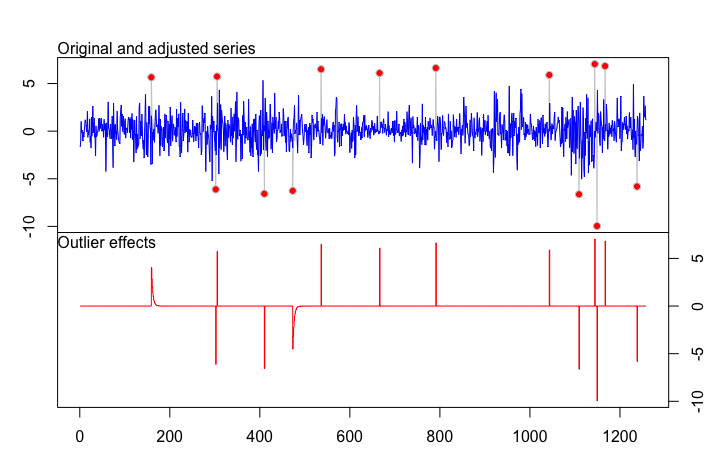
\includegraphics[width=0.50\textwidth]{\MainFolder/Images/Apoutliers.png}
\caption[\small Outliers detection for Apple Inc. daily closing return]{\small Outliers detection for Apple Inc.\@ daily closing return. The $x-$axis is labelled by the date index.}
\hrule\label{fig:apoutlier}
\end{figure}
\afterpage{\FloatBarrier}
\par The isolated sharp spikes represent AO, while a spike that takes a few periods to disappear represents a TC. Note that the $x-$axis is labelled by the time (date) index, not the actual date. The latter can easily be extracted using the following code:
\begin{lstlisting}[language=R]
ots=out_tso$outliers
cbind.data.frame(type=ots$type,
    date=data[ots$ind,1])
\end{lstlisting}
yields  
\begin{verbatim}
   type     date       type     date
1  TC 2015-01-28    8  AO 2017-08-01
2  AO 2015-08-21    9  AO 2018-08-01
3  AO 2015-08-26   10  AO 2018-11-02 
4  AO 2016-01-27   11  AO 2018-12-26
5  TC 2016-04-27   12  AO 2019-01-03
6  AO 2016-07-27   13  AO 2019-01-30
7  AO 2017-02-01   14  AO 2019-05-13
\end{verbatim}
\end{Example}

\subsection{R Package: \texttt{anomalize}} In this section, we will show how to use  \verb|anomalize| to detect anomalies in time series data. The package is available on CRAN, with the latest version always available on github. \par It is recommended to first install the package from CRAN (so that the dependencies are also installed locally), then update the package using devtools as shown below:

\begin{lstlisting}[language=R]
install.packages('anomalize')
library(devtools)
install_github("business-science/anomalize")
library(anomalize)
library(tidyverse)
\end{lstlisting}
\newpage\noindent
The \verb|anomalize()| function is used to detect outliers in a distribution with no trend or seasonality for tidy data, and returns three columns: 
\begin{itemize}[noitemsep]
\item \texttt{remainder-l1} (lower limit for anomalies);
\item \texttt{remainder-l2} (upper limit for anomalies, and 
\item \texttt{anomaly} (Yes/No).
\end{itemize}
The first argument of the function is the ``tibble'' or ``tbl\_time`` object \verb|data|; the second argument is the column \verb|target|, to which the function is applied; the third is the anomaly detection \verb|method|, either \verb|iqr| \verb|geds|. 
\newl The \textbf{IQR method} (inter-quartile range $Q_3-Q_1$) is a generalization of Tukey's test (see Section 1). By defaults, the limits are set at 3 times the IQR above $Q_3$ and below $Q_1$ (corresponding to $\alpha=0.05$); anything beyond those limits is considered to be an anomalous observation. \par The alpha parameter can be adjusted; at $\alpha = 0.025$, the limits are 6 times the IQR above $Q_3$ and below $Q_1$, making it more difficult for data to be an anomaly. Conversely, $\alpha = 0.1$ contracts the limits to $1.5$ times the IQR above $Q_3$ and below $Q_1$, making it more likely that observations will be deemed anomalous. \par The IQR method does not depend on loops and is therefore fast and easily scaled, but it may not be as accurate in detecting anomalies since the high leverage anomalies can skew the centerline (median) of the IQR. \newl The \textbf{GESD method} (generlized extreme studentized deviate test) progressively eliminates outliers using a Student's $T-$test comparing the test statistic to a critical value. Each time an outlier is removed, the test statistic is updated. Once the test statistic drops below the critical value, all outliers are considered removed. \par The $\alpha$ parameter adjusts the width of the critical values. By default, $\alpha = 0.05$. Because this method involves continuous updating via a loop, it is slower than the IQR method. However, it tends to outperform IQR for outlier detection and removal. \newl Other arguments include \verb|max_anoms| (the maximum percentage of observations that can be identified as anomalies) and \verb|verbose| (boolean linked to the type of output). 
\begin{Example} In the previous sub-section, we used the function \verb|tsoutliers()| to detect outliers of daily closing return for one of the components of DJ30, namely Apple Inc. An alternative manner to detect anomalies in R is to use \verb+anomalize()+, as follows: 
\begin{lstlisting}
data_tb=data %>% as.tibble()
data_tb %>% 
    time_decompose(AAPL,
            method="stl",
            frequency=10,
            trend="auto") %>%
    anomalize(remainder,
            method="gesd",
            alpha=0.05,
            max_anoms=0.2) %>%
    plot_anomaly_decomposition()
\end{lstlisting}
The output is shown in Figure~\ref{fig:apanomalies},
\begin{figure}[t]
\centering
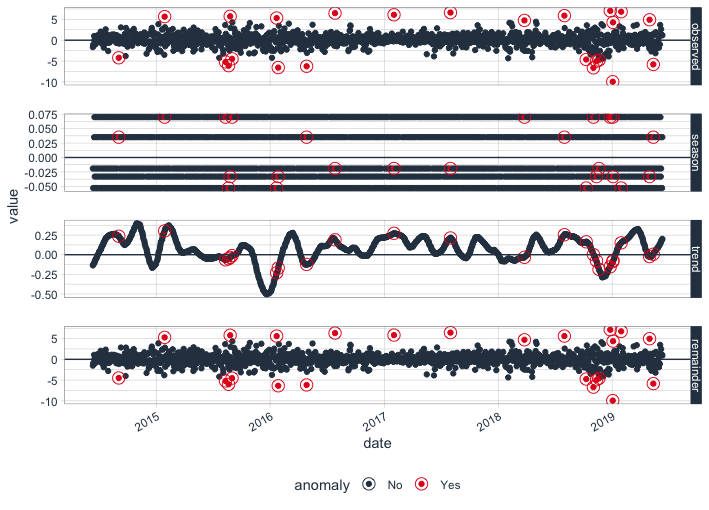
\includegraphics[width=0.5\textwidth]{\MainFolder/Images/Apanomalies.png}
\caption{\small Anomaly detection for Apple Inc.'s daily closing returns, computed with  \texttt{anomalize()}.}\label{fig:apanomalies}
\hrule
 \end{figure}
where the top plot displays the observations, the second and third plot displays the trend and seasonality components, respectively, and the bottom plot displays the extracted data on which anomalies are detected. The red markers show  the anomalies found by \verb|anomalize()|. The recomposed series can also be plotted \textit{via} \verb|time_recomposed()|:
\begin{lstlisting}
data_tb %>% time_decompose(AAPL) %>% 
  anomalize(remainder) %>% 
  time_recompose() %>%  
  plot_anomalies(time_recomposed=TRUE,
            ncol=3,
            alpha_dots=0.5)
\end{lstlisting}
The output is shown in Figure~\ref{fig:apanomaliesrecomp}.
\begin{figure}[t]
\centering
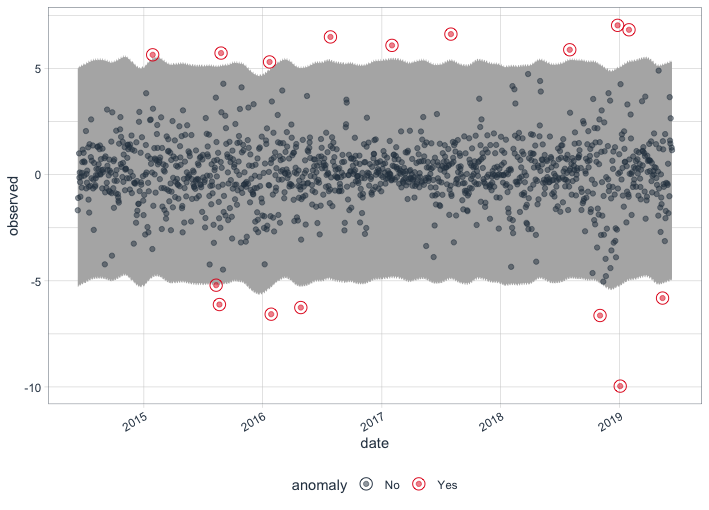
\includegraphics[width=0.5\textwidth]{\MainFolder/Images/Apanomaliesrecomp.png}
\caption{\small Anomaly detection for Apple Inc.'s daily closing returns with recomposed data; the grey portion represent the expected (normal) trend.}
\hrule\label{fig:apanomaliesrecomp}
\end{figure}
Anomalous points that are shown in red can be extracted by the following code:
\begin{lstlisting}
anomalies=data_tb %>%  
time_decompose(AAPL) %>%  
 anomalize(remainder) %>%  
 time_recompose() %>%  
 filter(anomaly=='Yes')
\end{lstlisting}
The output is a time tibble with 16 rows (with \verb|date| and \verb|observed| as the first two variables); these are the 16 observations that \verb|anomalize()| reports. Recall that in previous section, \verb|tsoutliers()| detected 14 outliers. \newl It is interesting to compare the outlier/anomaly dates for Apple Inc. data from both approaches. This can be done with the code on the following page:
\begin{lstlisting}
odates=cbind.data.frame(type=ots$type,
                 date=data[ots$ind,1])
adates=cbind.data.frame(date=anomalies$date,
          observed=anomalies$observed)
left_join(adates,odates,by="date")
\end{lstlisting}
The list of detected outliers is found below:
\begin{verbatim}
         date observed type
 1 2015-01-28    5.653   TC
 2 2015-08-11   -5.204 <NA>
 3 2015-08-21   -6.116   AO
 4 2015-08-26    5.735   AO
 5 2016-01-22    5.317 <NA>
 6 2016-01-27   -6.571   AO
 7 2016-04-27   -6.258   TC
 8 2016-07-27    6.496   AO
 9 2017-02-01    6.098   AO
10 2017-08-01    6.629   AO
11 2018-08-01    5.891   AO
12 2018-11-02   -6.633   AO
13 2018-12-26    7.042   AO
14 2019-01-03   -9.961   AO
15 2019-01-30    6.833   AO
16 2019-05-13   -5.812   AO
\end{verbatim}
All the observations that have been detected by the original approach (\verb|tsoutliers()|) match the ones reported by this new approach (\verb|anomalize()|), but \verb|anomalize()| also detects two extra points, for which the type cannot be specified. The comparison is also illustrated in Figure~\ref{fig:comparemethods}.
\begin{figure}[t]
\centering
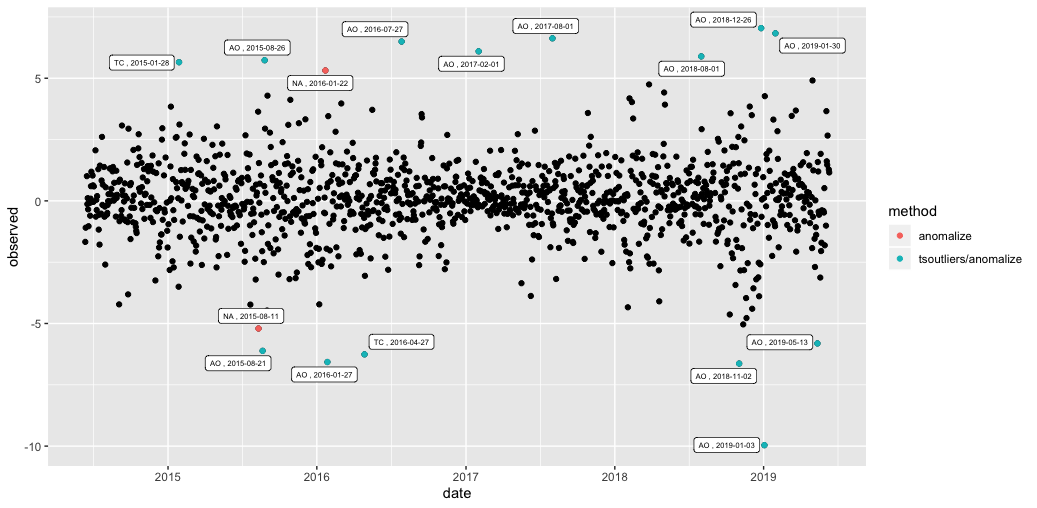
\includegraphics[width=0.5\textwidth]{\MainFolder/Images/comparemethods.png}
\caption{\small Comparing two methods of outlier/anomaly detection for Apple Inc.'s  daily closing returns.}
\hrule\label{fig:comparemethods}
\end{figure}
\end{Example}\afterpage{\FloatBarrier}

\subsection{Summary}
For time series data, anomaly detection is usually performed on time series \textbf{remainders}, where both the  \textbf{seasonal} and the \textbf{trend} components were removed; the former is the presence of variations that occur at specific regular intervals shorter than a year, such as daily, weekly, monthly, or quarterly while the later consists of longer term growth patterns. \newl The first task in the anomaly detection of a time series is thus to generate its remainders. 
\par There are different ways to decompose a time series to produce remainders: ARIMA and X12 are popular algorithms to do so.\footnote{\texttt{tsoutliers()} uses ARIMA while \texttt{anomalize()} uses seasonal decomposition.} \newl In general, high performance machine learning techniques are not recommended for anomaly detection since the overfitting reduces the difference between the observed and fitted values whereas in anomaly detection this difference is essential to highlight the anomaly. \par On the other hand, seasonal decomposition performs best for this task by removing the right features (i.e. seasonal and trend components) while preserving the characteristics of anomalies in the remainders. \newl Finally, we note that there are other popular R outlier analysis packages in R, such as \verb|AnomalyDetection|, which uses a method similar to \verb|anomalize|'s GESD. Interested readers are invited to try this package and compare their results with the functions reviewed in this section. 

%\subsection{More applications}
